% =====================================================================
%  ViralJEPA -- Deep Learning course project report, University of Padova
%  Compile with pdfLaTeX + BibTeX (Overleaf: default settings are fine).
%  Needs: references.bib, figures/exp04_finetune_curves.png
% =====================================================================
\documentclass[10pt,twocolumn,a4paper]{article}

\usepackage[utf8]{inputenc}
\usepackage[T1]{fontenc}
\usepackage{lmodern}
\usepackage[margin=1.8cm]{geometry}
\usepackage{microtype}
\usepackage{amsmath,amssymb}
\usepackage{graphicx}
\usepackage{tikz}
\usetikzlibrary{arrows.meta}
\usepackage{booktabs}
\usepackage{tabularx}
\usepackage{caption}
\usepackage{xcolor}
\usepackage[numbers,sort&compress]{natbib}
\usepackage[colorlinks=true,linkcolor=blue!45!black,citecolor=blue!45!black,
            urlcolor=blue!45!black]{hyperref}

\captionsetup{font=small,labelfont=bf}
\setlength{\parskip}{0.2em}
\setlength{\columnsep}{6mm}
\setlength{\bibsep}{0pt plus 0.2ex}        % tighter reference list
\setlength{\textfloatsep}{10pt plus 2pt minus 2pt}
\setlength{\dblfloatsep}{10pt plus 2pt minus 2pt}
\setlength{\dbltextfloatsep}{12pt plus 2pt minus 2pt}
\bibliographystyle{unsrtnat}

\begin{document}

% Title set across both columns.
\twocolumn[{%
\begin{center}
  {\LARGE\bfseries ViralJEPA: Same-Genome Self-Supervised Pretraining\\[3pt]
   for Detecting Unseen Viral Families in Human Metagenomes\par}
  \vspace{8pt}
  {\large Luca Grigolin\par}
  \vspace{3pt}
  {\small Deep Learning, University of Padova\par}
\end{center}
\vspace{10pt}
}]

% =====================================================================
\section{Introduction}
% =====================================================================

Metagenomic sequencing of a clinical sample returns DNA from everything the
specimen contained: the human host, its bacteria, and any viruses present.
Assigning the assembled contigs to an origin is normally done by alignment
against reference databases, but a large fraction of viral sequence matches
nothing known, the problem called viral dark
matter~\cite{krishnamurthy2017darkmatter}. Alignment-free classifiers instead
learn what viral sequence \emph{looks like}: VirFinder~\cite{ren2017virfinder}
works from $k$-mer frequencies, DeepVirFinder~\cite{ren2020deepvirfinder} and
Seeker~\cite{auslander2020seeker} apply neural networks to raw sequence, and
VirSorter2~\cite{guo2021virsorter2} and geNomad~\cite{camargo2024genomad}
combine learned signals with protein markers.

\paragraph{ViraMiner and ViraMiner-CB.}
\citet{tampuu2019viraminer} framed the task on human clinical metagenomes, with
contigs from several sample types cut into short windows and labelled by BLAST,
only a small fraction of them viral. Their network combines a \emph{pattern}
branch, asking whether a motif is present, with a \emph{frequency} branch,
asking how often motifs occur, and reaches a test AUROC of 0.923. A second
experiment holds out every anellovirus from training; since anelloviruses are
diverse, ubiquitous commensals of the human
virome~\cite{kaczorowska2020anello}, this unseen family is a meaningful probe of
generalisation. A later project of this course~\cite{pivotto2024viraminercb}
added an Inception-style first layer~\cite{szegedy2015inception} on the same
data and matched ViraMiner without surpassing it. Both datasets and splits are
reused unchanged here.

\paragraph{What this project adds.}
Both models are supervised convolutional networks trained on very few positives.
This project explores two ways to go beyond them. The first is architectural: a
convolution only sees a local window, whereas a
Transformer~\cite{vaswani2017attention} placed on top of convolutional motif
tokens can relate motifs anywhere in the sequence, combining the local pattern
detection of a CNN with global context. The second concerns the data: labelled
viral contigs are scarce, while unlabeled genomes are abundant, which is exactly
the asymmetry self-supervised pretraining
exploits~\cite{ji2021dnabert,zhou2024dnabert2,dallatorre2025nt,nguyen2023hyenadna}.
A joint-embedding predictive architecture (JEPA) pretrains the encoder by
predicting the representations of hidden parts of a sequence from the visible
ones, rather than the nucleotides themselves, so that it can learn what is
characteristic of a genome before seeing any label, and potentially carry that
knowledge to viral families absent from the labelled data.
The report presents a CNN--Transformer baseline (Section~\ref{sec:vm3}), the
case for a joint-embedding predictive objective (Section~\ref{sec:why}), a
leakage-controlled corpus (Section~\ref{sec:corpus}), the pretraining method and
the failed runs that shaped it (Section~\ref{sec:method}), the evaluation
protocol (Section~\ref{sec:eval}), the results of the final run
(Section~\ref{sec:results}) and the directions that would most improve the
pretraining (Section~\ref{sec:improve}). All code is
public~\cite{grigolin2026viraminer3,grigolin2026corpus,grigolin2026viraljepa}.

% =====================================================================
\section{ViraMiner3: a CNN--Transformer baseline}\label{sec:vm3}
% =====================================================================

\paragraph{Architecture and training.}
A one-hot sequence of shape $300\times4$ enters a multi-kernel stem: four Conv1D
layers in parallel with kernels of 5, 7, 11 and 15\,bp, 72 filters each, stride
2, GELU~\cite{hendrycks2016gelu}, concatenated into 150 tokens of 288 features
and normalised with BatchNorm~\cite{ioffe2015batchnorm}. The kernels span short
motifs up to about five codons, so the stem plays the role of ViraMiner's two
branches at several scales at once. A learned CLS token and learned positions are
added and a 6-layer pre-norm~\cite{xiong2020prenorm} Transformer (8 heads, width
288) mixes the tokens; the CLS output passes a LayerNorm~\cite{ba2016layernorm}
and an MLP ($288\to512\to128\to1$), for 6.3\,M parameters. Because positives are
rare the loss is focal~\cite{lin2017focal} ($\alpha=0.75$, $\gamma=2$, smoothing
0.05). AdamW~\cite{loshchilov2019adamw} uses $10^{-4}$ for the stem and head and
$5\cdot10^{-5}$ for the Transformer, which is frozen for 5 epochs so the random
head cannot push large gradients into the attention layers; the schedule is a
5-epoch warm-up then cosine decay~\cite{loshchilov2017sgdr}, at most 120 epochs,
patience 15 on validation AUROC, batch 128, fp16~\cite{micikevicius2018mixed}.
Augmentation is a reverse complement at probability 0.5 and a shift of up to
$\pm5$\,bp, since strand and cut points carry no label information. The operating
threshold maximises F1 on validation.

\paragraph{Choosing the baseline.}
A controlled trial compared this architecture with four variants changing either
the motif encoder or the token aggregation (Table~\ref{tab:vm3}). Shrinking the
stem to two kernels costs a point of AUROC, so the range of kernel sizes matters
more than filters per kernel; enlarging it to 512-dimensional tokens triples the
parameters and performs \emph{worse}, its collapse in precision (0.48) showing
the larger model overfitting a 2\%-positive training set. Local attention and
attention pooling leave test AUROC unchanged while lowering validation AUROC.
Neither component is the bottleneck, so the baseline was kept: at 0.932 it
improves on ViraMiner (0.923) and ViraMiner-CB (0.922) on the same split.

\begin{table*}[t]
\centering
\caption{ViraMiner3 architecture trial on the ViraMiner \texttt{fullset} test
split (551 viral contigs out of 26{,}405). Checkpoints are selected by validation
AUROC; precision, recall and F1 refer to the viral class at the best-F1
validation threshold. Single seed.}
\label{tab:vm3}
\footnotesize
\begin{tabular}{lrcccccc}
\toprule
Variant & Params & Val AUROC & Test AUROC & Test AP & Prec. & Rec. & F1 \\
\midrule
\textbf{Baseline: 4 kernels $\times$ 72, CLS} & 6.27\,M & \textbf{0.931} & \textbf{0.932} & 0.563 & 0.672 & \textbf{0.465} & \textbf{0.549} \\
Local attention, $\pm64$ tokens            & 6.27\,M & 0.926 & 0.930 & \textbf{0.566} & 0.683 & 0.437 & 0.533 \\
CLS $+$ attention pooling                  & 6.41\,M & 0.926 & 0.932 & 0.560 & \textbf{0.695} & 0.434 & 0.534 \\
2 kernels (7, 11) $\times$ 144             & 6.26\,M & 0.921 & 0.927 & 0.528 & 0.636 & 0.416 & 0.503 \\
4 kernels $\times$ 128, token width 512    & 19.34\,M & 0.920 & 0.925 & 0.517 & 0.484 & 0.454 & 0.468 \\
\midrule
ViraMiner~\cite{tampuu2019viraminer}       & --- & --- & 0.923 & --- & 0.90 & 0.32 & --- \\
ViraMiner-CB~\cite{pivotto2024viraminercb} & --- & --- & 0.922 & --- & 0.84 & 0.32 & --- \\
\bottomrule
\end{tabular}
\end{table*}

% =====================================================================
\section{Why a joint-embedding predictive objective}\label{sec:why}
% =====================================================================

Genomic foundation models are mostly pretrained by reconstructing their input:
DNABERT~\cite{ji2021dnabert}, DNABERT-2~\cite{zhou2024dnabert2} and the
Nucleotide Transformer~\cite{dallatorre2025nt} predict masked tokens,
HyenaDNA~\cite{nguyen2023hyenadna} and Evo~\cite{nguyen2024evo} the next
nucleotide. At single-base resolution DNA is close to incompressible, so such
losses spend much of their capacity on base-level detail, while the signal that
separates viral from host sequence lies in organism-level regularities such as
the genomic signature of oligonucleotide
composition~\cite{karlin1995signature}.

Joint-Embedding Predictive Architectures~\cite{lecun2022path} instead predict the
\emph{representation} of a hidden part of the input, letting the model discard
detail it cannot predict. Three works shape this project.
I-JEPA~\cite{assran2023ijepa} predicts the latent features of masked blocks from
a visible context, with targets from an exponential-moving-average (EMA) copy of
the encoder; data2vec~\cite{baevski2022data2vec} averages the top layers of that
teacher into a richer target; and JEPA-DNA~\cite{larey2026jepadna} brings the
idea to genomics, adding a latent objective on top of the generative loss.
Latent-matching objectives share one failure mode, collapse to constant or
low-rank outputs~\cite{jing2022dimensional}, which BYOL~\cite{grill2020byol}
counters with an asymmetric predictor and a slowly moving target and
VICReg~\cite{bardes2022vicreg} with explicit variance and covariance terms.
Finally, DNABERT-S~\cite{zhou2024dnaberts} showed that two fragments of one
genome make a natural positive pair, yielding embeddings that cluster by
species, the coarse distinction a viral classifier needs.

% =====================================================================
\section{The pretraining corpus}\label{sec:corpus}
% =====================================================================

What the unlabeled data contains is a design decision as consequential as the
objective. The corpus built for this project~\cite{grigolin2026corpus},
\texttt{corpus\_v3}, holds 4{,}000{,}000 windows of 300\,bp, matching the
downstream input length exactly so that no change of resolution occurs between
pretraining and fine-tuning. Three requirements shaped it: span the sequence
domains a human metagenome actually contains, on both sides of the decision;
contain no evaluation sequence, or a frozen probe would measure memorisation; and
leave one viral family completely unseen, preserving the anellovirus benchmark as
a genuine test of generalisation to a new taxon.

\subsection{Sources}

Five public reference collections were used (Table~\ref{tab:sources}), each
chosen to fill a specific gap. \emph{RefSeq viral}~\cite{oleary2016refseq} gives
broad taxonomic coverage of curated viral genomes; records whose description
mentions a phage are routed to the prokaryotic-virus category and the rest to the
eukaryotic one. \emph{NCBI Virus}~\cite{hatcher2017ncbivirus} adds depth where RefSeq is thin: complete genomes annotated with a human host, restricted to fourteen
families occurring in clinical metagenomes plus the human retroviruses. Public
archives are heavily skewed towards a few intensively sequenced species, so at
most ten genomes are kept per ICTV species; without this cap a handful of
pathogens would dominate the category. \emph{UHGV}~\cite{camargo2025uhgv}, the
unified human gut virome catalogue, contributes the phages that dominate real gut
samples and that RefSeq represents poorly~\cite{shkoporov2019phages}, restricted
to representatives rated \emph{Complete} or \emph{High-quality} by
CheckV~\cite{nayfach2021checkv} so that fragmentary assemblies do not enter as if
they were genomes.

The negatives come from two sources. \emph{UHGG}~\cite{almeida2021uhgg} supplies
1{,}000 gut species representatives at completeness $\ge90\%$ and contamination
$\le5\%$, selected round-robin across phyla so Firmicutes and Bacteroidota do not
crowd out the rest. \emph{T2T-CHM13v2.0}~\cite{nurk2022t2t} supplies human
sequence; the complete assembly was preferred because it resolves centromeres and
satellite arrays absent from GRCh38 that appear readily in real data and that a
classifier must learn not to flag. Finally 180{,}000 windows come from
\texttt{fullset\_train} with labels discarded, carrying the sequencing artefacts
and error profile of the target domain that no reference genome reproduces.

\begin{table*}[t]
\centering
\caption{Sources of \texttt{corpus\_v3}. Records and Mbp are counted after
filtering. The two virus categories draw on RefSeq and on NCBI Virus or UHGV
jointly, so their window counts are reported in Table~\ref{tab:mix} rather than
per source.}
\label{tab:sources}
\footnotesize
\begin{tabularx}{\textwidth}{llXr}
\toprule
Source & Category & Records kept & Records / Mbp \\
\midrule
RefSeq viral & virus, euk.\ and prok. & all, minus 175 anellovirus records and 139 duplicated in NCBI Virus & 19{,}275 / 580 \\
NCBI Virus & virus, eukaryotic & complete genomes, human host, $\le10$ per ICTV species; Anelloviridae dropped & 1{,}266 / 33 \\
UHGV & virus, prokaryotic & vOTU representatives of CheckV quality Complete or High-quality; 927 Anelloviridae dropped & 57{,}734 / 2{,}598 \\
UHGG v2.0.2 & bacteria & 1{,}000 species representatives, $\ge90\%$ complete, $\le5\%$ contaminated, balanced over phyla & 92{,}449 contigs / 2{,}612 \\
T2T-CHM13v2.0 & human & all 25 sequences of the analysis set & 25 / 3{,}117 \\
ViraMiner train & ViraMiner & random rows of \texttt{fullset\_train}, labels removed & --- \\
\bottomrule
\end{tabularx}
\end{table*}

\subsection{Window extraction and composition}

Each category receives a fixed share of the four million windows
(Table~\ref{tab:mix}). Viruses take just over half the corpus although they are a
small minority of any real sample: the encoder should model viral sequence well,
and the class prior belongs to the fine-tuned classifier, not to the pretraining
distribution. Within a category, windows are allocated to genomes in proportion
to length, capped at 50\,kb for every non-human source. Without the cap, jumbo
phages and poxviruses, two or three orders of magnitude longer than a
circovirus, would absorb most of the budget.

Windows are drawn at uniformly random positions. A window containing any
character outside ACGT is redrawn, up to four attempts, so that masking and
one-hot encoding stay well defined; soft-masked repeats are upper-cased and
retained, because repetitive human sequence is exactly what the model must learn
not to flag. Every window is reverse-complemented with probability 0.5, since a
contig may be sequenced from either strand. Each window keeps an identifier
\texttt{category|source|record|start|strand}. The \texttt{record} field, naming
the genome, contig or chromosome the window came from, is what makes the
paired-view objective of Section~\ref{sec:cls} possible: it is the only grouping
information the model ever receives, and the category is never exposed to it.

\begin{table*}[t]
\centering
\begin{minipage}[t]{0.45\textwidth}
\centering
\caption{Composition of \texttt{corpus\_v3}.}
\label{tab:mix}
\small
\begin{tabular}{lrr}
\toprule
Category & Share & Windows \\
\midrule
Viruses, prokaryotic & 32.5\% & 1{,}300{,}000 \\
Human                & 25.0\% & 1{,}000{,}000 \\
Bacteria, gut        & 20.0\% &   800{,}000 \\
Viruses, eukaryotic  & 18.0\% &   720{,}000 \\
ViraMiner, unlabeled &  4.5\% &   180{,}000 \\
\midrule
Total                & 100\%  & 4{,}000{,}000 \\
\bottomrule
\end{tabular}
\end{minipage}\hfill
\begin{minipage}[t]{0.52\textwidth}
\centering
\caption{Leakage screens. A window is discarded when at least 10\% of its
canonical $k$-mers occur in the screen set.}
\label{tab:screen}
\small
\begin{tabular}{p{2.2cm}p{2.5cm}cr}
\toprule
Applied to & Screen set & $k$ & Removed \\
\midrule
External genomes & \texttt{fullset} val.\ and test, anell.\ test & 31 & 95{,}340 \\
ViraMiner windows & anellovirus test split & 31 & 25{,}829 \\
All windows & anellovirus test positives & 15 & 447 \\
\bottomrule
\end{tabular}
\end{minipage}
\end{table*}

\subsection{Leakage control}

Any window reproducing an evaluation contig would let a probe or a fine-tuned
model score well for the wrong reason. Windows are therefore screened against
sets of canonical $k$-mers and discarded when at least 10\% of their $k$-mers
appear in the screen set (Table~\ref{tab:screen}). At $k=31$ this fires on
near-exact overlap while chance matches are effectively impossible. Most removals
are human windows (93{,}397), as expected since the non-viral part of ViraMiner
is largely human; because the anellovirus test split re-partitions the same pool
as \texttt{fullset\_train}, the ViraMiner-derived windows were screened against
it separately, removing a further 25{,}829.

Anelloviruses are excluded three times over: by taxonomic annotation, by a
regular expression over record descriptions, and by a screen at $k=15$ against
the anellovirus test positives. The shorter word is deliberate, since 15-mers
survive roughly 10\% divergence often enough to exceed the threshold while chance
matches stay at 1--2\% of a window, which catches relatives of the test family
that taxonomy alone would miss. The draw runs at 1.3 times the target count to
absorb these rejections, and the survivors are trimmed and shuffled.

Three limitations remain. RefSeq contains plant and insect viruses that never
occur in human samples; the per-species cap is taxonomic rather than
sequence-based, so near-identical strains can still repeat; and every bacterial
genome comes from the gut, while ViraMiner also draws on skin and cervical
samples, so the bacterial negatives are narrower than those met at test time.

% =====================================================================
\section{ViralJEPA}\label{sec:method}
% =====================================================================

\subsection{Architecture overview}\label{sec:arch}

ViralJEPA pretrains the encoder that will later be fine-tuned, a CNN stem
followed by a Transformer, by combining a token-level JEPA with a sequence-level
objective on the CLS token (Figure~\ref{fig:arch}). Each training example is a
pair of windows from the same record of the corpus. The \emph{context encoder}
reads window $A$ with parts of it hidden and is the only network trained by
gradient descent, together with its small heads. A \emph{target encoder}, an EMA
copy of it that receives no gradient, reads the clean $A$ to provide the targets
of the hidden tokens, and the clean $B$ to provide a target for the CLS. Four
signals train the context encoder: latent prediction of the hidden spans and
base-level prediction of scattered hidden tokens on the token side
(Section~\ref{sec:tokobj}), and on the CLS side a prediction of the other
window's embedding, kept from collapsing by variance and covariance terms, and of
its 4-mer composition (Section~\ref{sec:cls}).

\begin{figure*}[t]
\centering
\resizebox{\textwidth}{!}{%
\begin{tikzpicture}[
  >={Stealth[length=2mm]}, font=\scriptsize,
  box/.style={draw, rounded corners=2pt, align=center, text width=2.75cm,
              minimum height=0.8cm, inner sep=3pt},
  loss/.style={box, fill=black!8},
  data/.style={box, dashed},
  lab/.style={font=\scriptsize\itshape, inner sep=1pt}]
% columns: 0, 3.4, 6.8, 10.2, 13.6
% --- target branch for the tokens (top)
\node[data] (cA)   at (0,3)     {Window $A$, clean};
\node[box]  (tenc) at (6.8,3)   {Target encoder\\EMA copy, no gradient};
\node[box]  (ytgt) at (10.2,3)  {Token targets $y_i$\\mean of last 3 blocks,\\LayerNorm};
% --- context branch (middle)
\node[data] (mA)   at (0,0)     {Window $A$, masked\\JEPA spans and scattered\\tokens set to N};
\node[box]  (stem) at (3.4,0)   {CNN stem\\kernels 5, 7, 11, 15 $\times$ 72,\\stride 2, LayerNorm\\$\to$ 150 tokens $\times$ 288};
\node[box]  (ctx)  at (6.8,0)   {Context encoder\\CLS, mask token, positions\\6-layer Transformer,\\8 heads};
\node[box]  (pred) at (10.2,1.5){Predictor $g_\phi$\\4 layers, width 144,\\3 heads};
\node[box]  (mlm)  at (10.2,0)  {MLM head\\linear};
\node[loss] (Lj)   at (13.6,1.5){$\mathcal{L}_{\text{jepa}}$\\MSE on span tokens};
\node[loss] (Lm)   at (13.6,0)  {$\mathcal{L}_{\text{mlm}}$\\cross-entropy on\\scattered tokens};
% --- CLS branch (bottom)
\node[loss] (Lvc)  at (3.4,-1.7){$\mathcal{L}_{\text{var}}+\mathcal{L}_{\text{cov}}$\\VICReg on $z_A$};
\node[box]  (proj) at (6.8,-1.7){Projector $h$\\MLP to 1024};
\node[box]  (q)    at (10.2,-1.7){Predictor $q$};
\node[loss] (Lg)   at (13.6,-1.7){$\mathcal{L}_{\text{global}}$\\$1-\cos$};
\node[box]  (kh)   at (10.2,-3.1){4-mer head\\linear};
\node[loss] (Lk)   at (13.6,-3.1){$\mathcal{L}_{\text{kmer}}$\\KL divergence};
\node[data] (cB)   at (0,-4.6)  {Window $B$, clean\\same record as $A$};
\node[box]  (tencB)at (6.8,-4.6){Target encoder\\and projector $\bar h$\\EMA, no gradient};
\node[box]  (prof) at (10.2,-5.9){4-mer profile of $B$\\both strands};
% --- arrows: tokens
\draw[->] (cA) -- (tenc);
\draw[->] (tenc) -- (ytgt);
\draw[->] (ytgt.east) -| node[lab, pos=0.75, right] {sg} (Lj.north);
\draw[->] (mA) -- (stem);
\draw[->] (stem) -- (ctx);
\draw[->, dashed] (ctx.north) -- node[lab, right] {EMA} (tenc.south);
\draw[->] (ctx.east) -- node[lab, above] {tokens} (mlm.west);
\draw[->] (8.5,0) |- (pred.west);
\draw[->] (pred) -- (Lj);
\draw[->] (mlm) -- (Lm);
% --- arrows: CLS
\draw[->] (ctx.south) -- node[lab, left, pos=0.4] {CLS $c_A$} (proj.north);
\draw[->] (proj) -- node[lab, above] {$z_A$} (q);
\draw[->] (proj) -- (Lvc);
\draw[->] (q) -- (Lg);
\draw[->] (6.8,-0.9) -- (8.5,-0.9) |- (kh.west);
\draw[->] (kh) -- (Lk);
\draw[->] (cB) -- (tencB);
\draw[->] (tencB.east) -- (15.7,-4.6) |- node[lab, pos=0.25, right] {sg} (Lg.east);
\draw[->] (cB.south) |- (prof.west);
\draw[->] (prof.east) -| (Lk.south);
\end{tikzpicture}}
\caption{ViralJEPA pretraining. The context encoder reads window $A$ with JEPA
spans and scattered tokens hidden; an EMA copy of it reads the clean $A$ and the
clean $B$, a second window of the same record, and provides targets under a
stop-gradient (sg). Token side: a predictor regresses the target tokens of the
hidden spans and a linear head recovers the bases of the scattered tokens. CLS
side: the projected CLS must predict the target's projection of $B$, carries the
VICReg variance and covariance terms, and a linear head predicts the 4-mer
profile of $B$. Shaded boxes are loss terms; only the context encoder and its
heads receive gradients.}
\label{fig:arch}
\end{figure*}

\subsection{Encoder and masking}

The encoder is the ViraMiner3 architecture of Section~\ref{sec:vm3} with a
LayerNorm stem and the CLS token kept \emph{inside} the Transformer, exactly
where the classifier will read it. Two kinds of token are hidden from the context
encoder; each token covers 2\,bp.

\textbf{JEPA spans} are contiguous and non-overlapping, on a schedule growing
linearly from one or two spans covering 10--20\% of the tokens to one to four
covering 20--30\%. Span masking follows SpanBERT~\cite{joshi2020spanbert}, the
block masking of I-JEPA~\cite{assran2023ijepa} and the scheduler of
JEPA-DNA~\cite{larey2026jepadna}, whose ratios reach 50\%; they were lowered
because on a 150-token window a 50\% span hides 150 consecutive bases, half the
contig, leaving a context too thin to predict from.

\textbf{Scattered MLM tokens} are single tokens outside the spans, each hidden
with probability 0.15 as in BERT~\cite{devlin2019bert}, so their neighbours stay
visible and their bases remain predictable from local context. This corrects
exp02, where the MLM loss was scored inside the long spans and never improved on
base frequencies: the middle of a 150\,bp gap carries no recoverable local
information for a single-nucleotide model trained from scratch.

About 28\% of tokens are hidden at the start of training and 36\% at the end.
Hidden bases are set to N \emph{before} the stem, so no visible token's
overlapping kernel can see them, and the tokens are replaced by a learnable mask
embedding \emph{after} it, as in BERT and MAE~\cite{he2022mae}. The CLS token is
never masked.

\subsection{Token objective: latent prediction of the hidden spans}\label{sec:tokobj}

The target encoder is an EMA copy of the context encoder,
$\bar\theta\leftarrow m\,\bar\theta+(1-m)\,\theta$, with $m$ rising linearly from
0.996 to 1 as in BYOL and I-JEPA; it sees the unmasked window $A$. Following
data2vec~\cite{baevski2022data2vec}, the target $y_i$ for token $i$ is the
average of the outputs of the last $K=3$ Transformer blocks, each passed through
a LayerNorm without affine parameters, which gives a richer and more stable
target than the final layer alone. A narrow predictor $g_\phi$ (four pre-norm
layers at half the encoder width, three heads, fixed sinusoidal positions, as in
JEPA-DNA) receives the context CLS and tokens with mask embeddings at the hidden
positions and predicts each masked span token individually, as in I-JEPA:
\begin{equation}
\mathcal{L}_{\text{jepa}}
 =\frac{1}{|S|}\sum_{i\in S}\frac{1}{d}
   \bigl\lVert\, g_\phi\bigl(\mathrm{ctx}(A)\bigr)_i-\operatorname{sg}(y_i)\,\bigr\rVert_2^2 ,
\end{equation}
with $S$ the set of span tokens and $\operatorname{sg}$ the stop-gradient. Giving
every position its own target is what keeps the tokens apart: predicting 150
distinct vectors is impossible for an encoder whose tokens have collapsed onto
one, which is exactly the solution exp03 found. A linear MLM head on the context
tokens predicts the two bases under each scattered token by cross-entropy,
$\mathcal{L}_{\text{mlm}}$, keeping the tokens accurate at base level in the same
spirit as JEPA-DNA retaining the native generative loss.

\subsection{CLS objective: learning what windows of a genome share}\label{sec:cls}

The sequence-level objective is attached to the CLS token rather than to a pooled
summary of the tokens, mirroring DINO and iBOT~\cite{caron2021dino,zhou2022ibot},
where a global token carries the image-level objective and patch tokens the local
one. The CLS receives three signals.

\paragraph{A second view from the same genome.}
For each window $A$ a second window $B$ is drawn from the same record, and both
are augmented independently. $A$ and $B$ share no bases and may lie on opposite
strands, so what they have in common is a property of the organism: composition,
codon usage, GC skew. This is the positive pair of
DNABERT-S~\cite{zhou2024dnaberts}, playing the role of random crops in
SimCLR~\cite{chen2020simclr} and DINO; only record membership is used, never the
category. Single-window records, the ViraMiner rows, fall back to a re-augmented
copy of $A$.

\paragraph{Self-distillation, regularised on the projector.}
Following BYOL~\cite{grill2020byol}, the CLS of the masked $A$ passes through a
projector $h$ (an MLP to 1024 dimensions, with LayerNorm in place of BYOL's
BatchNorm, whose statistics would drift between the online and EMA copies) and a
predictor $q$, and must match the EMA target's projection of the
clean $B$:
\begin{equation}
\mathcal{L}_{\text{global}}
 = 1-\cos\!\bigl(q(h(c_A)),\ \operatorname{sg}\bigl(\bar h(\bar c_B)\bigr)\bigr).
\end{equation}
The asymmetric predictor and the slowly moving target keep this from collapsing
without negative pairs~\cite{tian2021understanding,chen2021simsiam}, and reading
the \emph{masked} $A$ forces the CLS to identify the organism from about 70\% of
the window. A VICReg variance hinge ($\gamma=1$ per dimension) and covariance
penalty act on the projector output $z_A=h(c_A)$, where
VICReg~\cite{bardes2022vicreg} prescribes them: the projector absorbs the
pressure to be spread out and decorrelated, leaving the CLS free to keep whatever
structure is useful.

\paragraph{A composition target.}
A linear head on the CLS of $A$ predicts the 4-mer profile of $B$, counted over
both strands, under a KL divergence. Computed from the DNA, this target cannot
collapse and is informative from the first step, unlike the early EMA target.
Predicting $B$'s profile rather than $A$'s prevents solving it by counting
visible bases, so the best prediction is the organism's average profile. As
MaskFeat~\cite{wei2022maskfeat} regresses HOG features, this aims the objective
at the genomic signature~\cite{karlin1995signature} that the $k$-mer baselines
rely on.

The total objective is
\begin{equation}
\mathcal{L}=\mathcal{L}_{\text{jepa}}+\mathcal{L}_{\text{global}}
           +\mathcal{L}_{\text{kmer}}+\mathcal{L}_{\text{mlm}}
           +\lambda_{v}\,\mathcal{L}_{\text{var}}+\lambda_{c}\,\mathcal{L}_{\text{cov}},
\end{equation}
with $\lambda_v=1$ and $\lambda_c=0.04$. Pretraining runs 60{,}000 steps at batch
512 (about 7.7 corpus passes) with AdamW, peak learning rate $5\cdot10^{-4}$,
3{,}000 warm-up steps then cosine decay, weight decay 0.05, gradient clipping at
1 and bf16. Each loss is logged beside the value it would take if the model
predicted the batch mean, so a term counts as informative only when it falls
clearly below that baseline.

% =====================================================================
\section{Evaluation protocol}\label{sec:eval}
% =====================================================================

The pretrained encoder is judged by a frozen linear probe, which asks what the
representation contains, and by full fine-tuning, which asks whether pretraining
helps the end task. Both compare against a randomly initialised encoder of the
same architecture and recipe, an essential control since a random encoder is
already a competitive $k$-mer feature extractor.

\paragraph{Frozen linear probe.}
A logistic regression is fitted on standardised, strand-averaged features of
clean \texttt{fullset\_train} windows and scored on \texttt{fullset\_test}, for
two read-outs: the CLS output, which the classifier uses, and the mean of the
token outputs. Besides AUROC and average precision, RankMe~\cite{garrido2023rankme}
measures the effective rank of the features, which drops sharply when the
representation collapses. The probe also runs every 5{,}000 pretraining steps
(Table~\ref{tab:probe}).

\paragraph{Fine-tuning.}
\texttt{fullset} trains on \texttt{fullset\_train}, selects on
\texttt{fullset\_validation} and reports on \texttt{fullset\_test} (551 viral of
26{,}405). \texttt{anell} trains on the anellovirus training split, minus windows
identical to a test window and a 10\% validation split, and reports on its test
split (1{,}348 viral of 27{,}644). It needs its own fine-tune because its test
positives also occur in \texttt{fullset\_train}, and since anelloviruses are
absent from the corpus, the fine-tuning data and the screens, it measures
transfer to an unseen family. The classifier is the encoder plus the MLP head of
Section~\ref{sec:vm3} on the CLS, trained as the supervised baseline with the
Transformer frozen for the first 5 epochs, the linear-probe-then-fine-tune order
that preserves pretrained features~\cite{kumar2022lpft}. Checkpoints are selected
on validation average precision, the more discriminating metric at 2\% positives.
Each task and initialisation runs with three seeds, with metrics reported plain
and with reverse-complement test-time averaging, and bootstrap 95\% confidence
intervals on test AUROC and AP (Table~\ref{tab:finetune}).

% =====================================================================
\section{Results}\label{sec:results}
% =====================================================================

The final run, \emph{exp04}, pretrained for 60{,}000 steps in 2.1\,h on a single
GPU and was then fine-tuned twelve times (two tasks, two initialisations,
three seeds), all in one job with the configuration of Section~\ref{sec:method}.

\begin{table}[t]
\centering
\caption{Frozen linear probe of exp04: fitted on \texttt{fullset\_train}, scored
on \texttt{fullset\_test}, reverse-complement averaged features of the EMA target
encoder. RankMe is out of 288.}
\label{tab:probe}
\footnotesize
\setlength{\tabcolsep}{4pt}
\begin{tabular}{llccc}
\toprule
Encoder & Read-out & AUROC & AP & RankMe \\
\midrule
Random init. & CLS       & 0.840 & 0.135 & 57.3 \\
Random init. & mean-pool & 0.843 & 0.125 & 47.8 \\
ViralJEPA    & CLS       & \textbf{0.912} & \textbf{0.375} & 158.8 \\
ViralJEPA    & mean-pool & 0.885 & 0.290 & \textbf{160.6} \\
\bottomrule
\end{tabular}
\end{table}

\subsection{The CLS objective: where the information ended up}\label{sec:res:cls}

Table~\ref{tab:probe} shows that pretraining put useful information into the
representation. A logistic regression on the frozen CLS reaches 0.912 test AUROC
against 0.840 for a random encoder, and average precision almost triples. A
\emph{linear} read-out of frozen features thus nearly matches the fully trained
ViraMiner network, although no label was seen during pretraining.

The sequence-level objective also put that information where the classifier
reads it. At initialisation the CLS and the mean of the tokens are within a
point of each other; after pretraining the CLS leads by 2.7 points of AUROC and
8.4 of AP. Both read-outs end with nearly the same effective rank, about 160 of
288, so what differs is not how much information each carries but whether the
viral/non-viral distinction is linearly accessible in it, the division of labour
borrowed from DINO and iBOT. The probe had nearly plateaued by the end of
pretraining, so longer training under this recipe would add little.

\begin{table*}[t]
\centering
\caption{Fine-tuning results of exp04, mean $\pm$ standard deviation over three
seeds. RC denotes reverse-complement test-time averaging; precision, recall and
F1 refer to the viral class at the best-F1 validation threshold. Checkpoint
selection differs between rows: the ViraMiner and ViraMiner3 checkpoints are
selected on best validation AUROC, the random and ViralJEPA ones on best
validation AP. The ViraMiner3 row is the single-seed supervised reference of
Table~\ref{tab:vm3} (BatchNorm stem, no RC averaging); the ViraMiner anellovirus
figure is that of its frequency branch, the best of its branches on that test
set~\cite{tampuu2019viraminer}.}
\label{tab:finetune}
\scriptsize
\setlength{\tabcolsep}{3.5pt}
\begin{tabular}{llcccccccc}
\toprule
Task & Init. & Seeds & AUROC & AP & AUROC RC & AP RC & F1 RC & Prec.\ RC & Rec.\ RC \\
\midrule
\texttt{fullset} & ViraMiner~\cite{tampuu2019viraminer} & 1 & 0.923 & --- & --- & --- & --- & --- & --- \\
\texttt{fullset} & ViraMiner3 & 1 & 0.932 & 0.563 & --- & --- & 0.549 & 0.672 & 0.465 \\
\texttt{fullset} & random     & 3 & $0.918\pm0.005$ & $0.573\pm0.005$ & $0.931\pm0.003$ & $0.617\pm0.005$ & $0.594\pm0.006$ & $\mathbf{0.775\pm0.047}$ & $0.484\pm0.023$ \\
\texttt{fullset} & ViralJEPA  & 3 & $\mathbf{0.932\pm0.005}$ & $\mathbf{0.598\pm0.007}$ & $\mathbf{0.942\pm0.005}$ & $\mathbf{0.625\pm0.011}$ & $\mathbf{0.601\pm0.010}$ & $0.740\pm0.024$ & $\mathbf{0.507\pm0.018}$ \\
\midrule
\texttt{anell}   & ViraMiner~\cite{tampuu2019viraminer} & 1 & 0.755 & --- & --- & --- & --- & --- & --- \\
\texttt{anell}   & random     & 3 & $0.791\pm0.003$ & $0.231\pm0.009$ & $0.822\pm0.007$ & $0.268\pm0.006$ & $0.182\pm0.007$ & $0.587\pm0.033$ & $0.108\pm0.006$ \\
\texttt{anell}   & ViralJEPA  & 3 & $\mathbf{0.875\pm0.024}$ & $\mathbf{0.455\pm0.023}$ & $\mathbf{0.895\pm0.019}$ & $\mathbf{0.491\pm0.030}$ & $\mathbf{0.380\pm0.048}$ & $\mathbf{0.755\pm0.030}$ & $\mathbf{0.257\pm0.047}$ \\
\bottomrule
\end{tabular}
\end{table*}

\begin{figure*}[t]
\centering
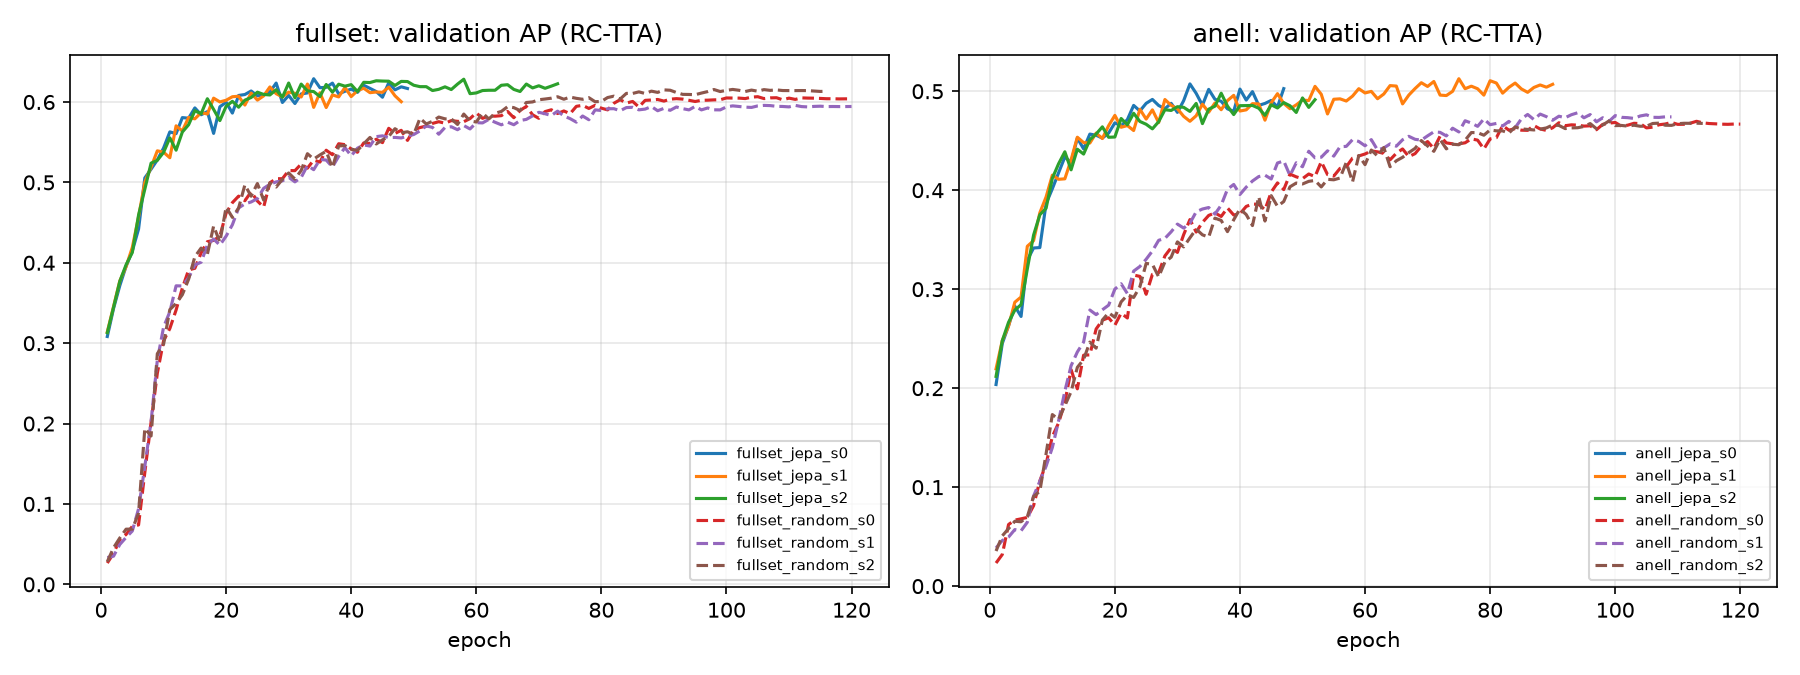
\includegraphics[width=0.90\textwidth]{figures/exp04_finetune_curves.png}
\caption{Validation average precision (RC-averaged) during fine-tuning, three
seeds per initialisation. ViralJEPA (solid) starts high while the Transformer is
still frozen and peaks in 32--75 epochs; the random encoder (dashed) needs
94--113 and three of its six runs reach the 120-epoch cap. Note that the \texttt{anell}
validation split contains no anelloviruses, so the right panel shows an
in-distribution gap of only about three points, much smaller than the
anellovirus test gap of Table~\ref{tab:finetune}.}
\label{fig:exp04ft}
\end{figure*}

\subsection{What the corpus-based self-supervision buys}\label{sec:res:ft}

Nothing in pretraining saw a label: the only supervision was which windows of
the corpus come from the same record. Fine-tuning asks what that is worth once
labels are available, and the two tasks answer differently.

\paragraph{Convergence.}
Pretraining changes how fine-tuning starts more than where it ends
(Figure~\ref{fig:exp04ft}). With the Transformer still frozen, the pretrained
encoder already reaches a validation AP above 0.41 on \texttt{fullset}, against
about 0.07 for the random one, and it reaches its best checkpoint two to three
times sooner.

\paragraph{In distribution.}
On \texttt{fullset} ViralJEPA improves on the random initialisation in every
seed-averaged metric (Table~\ref{tab:finetune}), but the gain is small and does
not survive a stricter comparison: three-seed ensembles of the two are
statistically indistinguishable under a paired bootstrap over test contigs.
Against the supervised references, ViralJEPA equals ViraMiner3's AUROC with
higher AP and F1 and, with RC averaging, exceeds ViraMiner. These references
select checkpoints on validation AUROC rather than AP, which tilts the AUROC
comparison towards them and the AP comparison towards ViralJEPA; the comparison
with the random control, which shares the protocol, is unaffected.

\paragraph{On an unseen family.}
The anellovirus task is where the corpus pays, and the effect is large.
Seed-averaged AUROC rises from 0.791 to 0.875 and AP nearly doubles, from 0.231
to 0.455, a factor of 1.97; with RC averaging, from 0.822 to 0.895 and from 0.268
to 0.491, a factor of 1.83. The three-seed ensembles reach 0.923 and 0.532 against 0.845 and 0.296, and the
paired bootstrap gives $+0.078$ $[0.069, 0.086]$ AUROC and $+0.234$
$[0.214, 0.257]$ AP, far from zero. At the best-F1 validation threshold the
classifier finds 26\% of the anellovirus contigs at 75\% precision, against 11\%
at 59\%, and at 90\% precision the ensemble still recovers 13\% of them where the
random ensemble recovers almost none (0.1\%). Every seed of ViralJEPA, including the weakest at
0.845 AUROC, is far above ViraMiner's 0.755 on the same test set; since
ViralJEPA is selected on AP and ViraMiner on AUROC, the selection protocol, if
anything, understates this AUROC margin.

The decisive observation is \emph{where} the gain appears. The \texttt{anell}
validation split is drawn from the anellovirus-free training data, and there the
two initialisations differ by only 3.3 points of AP (0.506 against 0.473), the
same small in-distribution margin as on \texttt{fullset}. On the anellovirus test
set the margin grows to 22 points. Pretraining therefore does not mainly make the
classifier better at the viruses it was trained on; it makes it generalise to a
family that no stage of the pipeline contained. Anelloviruses were kept out of
the corpus three times over, by taxonomic annotation, by a regular expression
over record descriptions and by a $k=15$ screen against the test positives
(Section~\ref{sec:corpus}), and out of the fine-tuning split as well. A
supervised encoder learns the specific viral families it is shown; the pretrained
one, having been asked four million times what two windows of one genome have in
common, carries a more general notion of viral sequence into fine-tuning.

\subsection{Has pretraining learned useful representations?}

Yes, and the two halves of the method can be credited separately. The CLS
objective decided \emph{where} the information sits: a read-out that was within a
point of mean pooling at initialisation ends 8.4 points of AP ahead of it, at
equal effective rank, and it is the read-out the classifier uses.
The corpus-based self-supervision decided \emph{what} was learned: pairing
windows by genome across four million windows of viral, bacterial and human
sequence produced a representation whose advantage shows up almost entirely out
of distribution, 22 points of AP on a family held out of every stage against 3
points in distribution. What the combination does not do is lift the
in-distribution ceiling. Once the random encoder is trained to convergence on
211{,}000 labelled windows, the two are statistically indistinguishable on
\texttt{fullset}.

% =====================================================================
\section{How the pretraining could be improved}\label{sec:improve}
% =====================================================================

Little of the remaining slack is in the compute budget: pretraining took 2.1
hours and the probe had nearly plateaued. The binding constraints are what a
positive pair means and how the objective is scheduled.

\begin{table}[t]
\centering
\caption{Record granularity in \texttt{corpus\_v3}. A record is what the
same-genome view of Section~\ref{sec:cls} samples from: a chromosome for human, a
genome for viruses, a UHGG contig for bacteria, a single window for the ViraMiner
rows. Pairing is informative only in the middle of this range.}
\label{tab:records}
\footnotesize
\setlength{\tabcolsep}{4pt}
\begin{tabular}{lrrr}
\toprule
Category & Records & Windows/record & Single-window \\
\midrule
Human                & 25      & 40{,}000 & 0 \\
Viruses, eukaryotic  & 14{,}100  & 51.1   & 31 \\
Viruses, prokaryotic & 63{,}701  & 20.4   & 1{,}237 \\
Bacteria, gut        & 83{,}675  & 9.6    & 11{,}132 \\
ViraMiner            & 180{,}000 & 1.0    & 180{,}000 \\
\midrule
Total                & 341{,}501 & 11.7   & 192{,}400 \\
\bottomrule
\end{tabular}
\end{table}

\paragraph{Make a positive pair mean the same thing in every category.}
Table~\ref{tab:records} shows how uneven the pairing is. For a virus the two
windows come from one genome of at most 50\,kb, a genuinely local relation; for a
human window the partner may lie hundreds of megabases away on the same
chromosome, and the constraint degenerates into ``both are human''. Splitting
human chromosomes and bacterial genomes into pseudo-records of about 50\,kb would
make \emph{same record} mean \emph{same neighbourhood} everywhere; a two-level
target weighting near and far pairs differently would go further.

\paragraph{Give the ViraMiner windows a real partner.}
The 180{,}000 windows closest to the target domain are exactly the ones that fall
back to a re-augmented copy of themselves. Yet ViraMiner identifiers decompose
into a contig and a piece index, and 44\% of \texttt{fullset\_train} rows belong
to a contig with at least one sibling, so grouping them by contig would give the
domain-matched data the same organism-level pairs, from data already in hand and
without using labels.

\paragraph{Warm up the self-distillation term.}
Early in training the EMA teacher places every window in nearly the same place,
so the cross-view loss has almost nothing to chase. Ramping in the weight of
$\mathcal{L}_{\text{global}}$ over the warm-up, while the 4-mer term shapes the
CLS, or starting the EMA momentum lower so the teacher tracks the student sooner,
would avoid the brief token collapse seen early in the run.

% =====================================================================
\section{Conclusions}\label{sec:conclusions}
% =====================================================================

This project asked whether self-supervised pretraining can push viral sequence
detection in human metagenomes beyond supervised training on the ViraMiner data.
Four conclusions follow.

\paragraph{Architecture gives a modest but real improvement.}
Replacing ViraMiner's pooled convolutional branches with convolutional motif
tokens and a Transformer raises test AUROC from 0.923 to 0.932, and no larger or
differently aggregated variant does better. The architecture was not the
bottleneck, which is what made the pretraining question worth asking.

\paragraph{Most of the real work is in the corpus, not the objective.}
Capping genomes by length and species keeps a few over-sequenced organisms from
defining what a virus looks like, and the $k$-mer screens keep the anellovirus
benchmark free of leakage, which is what makes its result credible. A
pretraining result is only as trustworthy as the leakage control behind it.

\paragraph{The same-genome objective works, and the two halves can be told apart.}
A CLS objective supervised by a second window of the same genome, alongside a
token-level latent objective, gives an encoder that clearly beats random
initialisation on a frozen probe. The CLS objective determined \emph{where} the
information sits, the read-out the classifier uses; the corpus-based pairing
determined \emph{what} was learned, and its benefit is almost entirely out of
distribution.

\paragraph{Pretraining is an accelerator in distribution and a generaliser out of it.}
On \texttt{fullset} the pretrained encoder matches the best supervised model in
two to three times fewer epochs, but with enough labels the random encoder ends
in the same place. On the held-out anellovirus family AUROC rises from 0.791 to
0.875 and average precision nearly doubles, well above ViraMiner's 0.755: the
encoder has learned something about viral sequence as such rather than about the
families it was trained on.

That is what matters for viral dark matter, sequence that by definition
resembles nothing in the databases: a classifier is useful there in proportion
to how well it transfers to families it has never seen, and that is where
pretraining helped most, at no labelling cost. The natural next steps
(Section~\ref{sec:improve}) are a positive pair that means the same thing across
the corpus, real second views for the domain-matched windows, and a gentler start
to the self-distillation term.

{\scriptsize
\bibliographystyle{unsrtnat}
\bibliography{references}
}

\end{document}
